\documentclass[class=NCU_thesis, crop=false]{standalone}
\usepackage[newfloat]{minted}
\usepackage{floatrow}
\usepackage{graphicx}


\begin{document}

\chapter{實驗設計與結果}

\section{實驗一:機械臂的基本控制}
\subsection{機械結構設計圖}
本實驗的硬體部分使用了3D列印技術,結合小型伺服馬達,設計了一個頂端為夾爪的小型機械臂,以下為此硬體的詳細設計圖紙:
\begin{figure}[htbp]
    \centering
    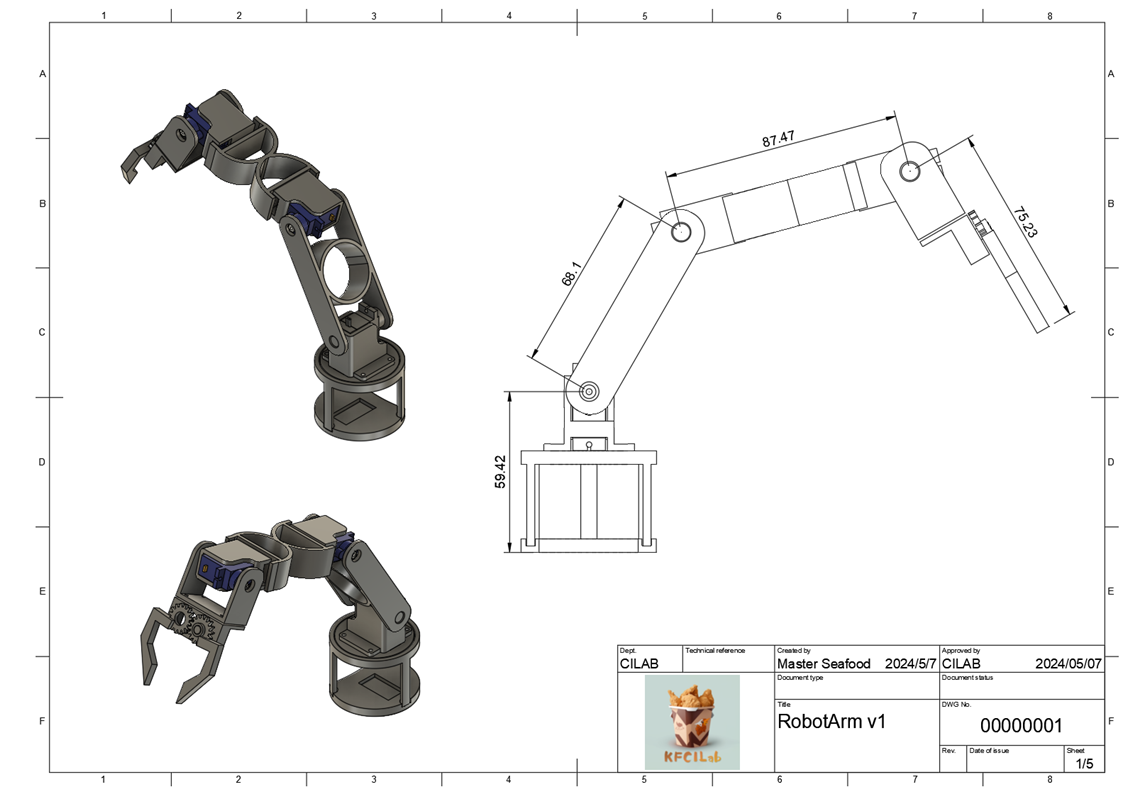
\includegraphics[width=0.9\textwidth]{figures/Armv1 (1).PNG}
    \caption{機械臂版本一設計圖紙 第一頁(單位:mm)}
    %\label{fig:Armv1Drawing_p1}}
\end{figure}

\begin{figure}[htbp]
    \centering
    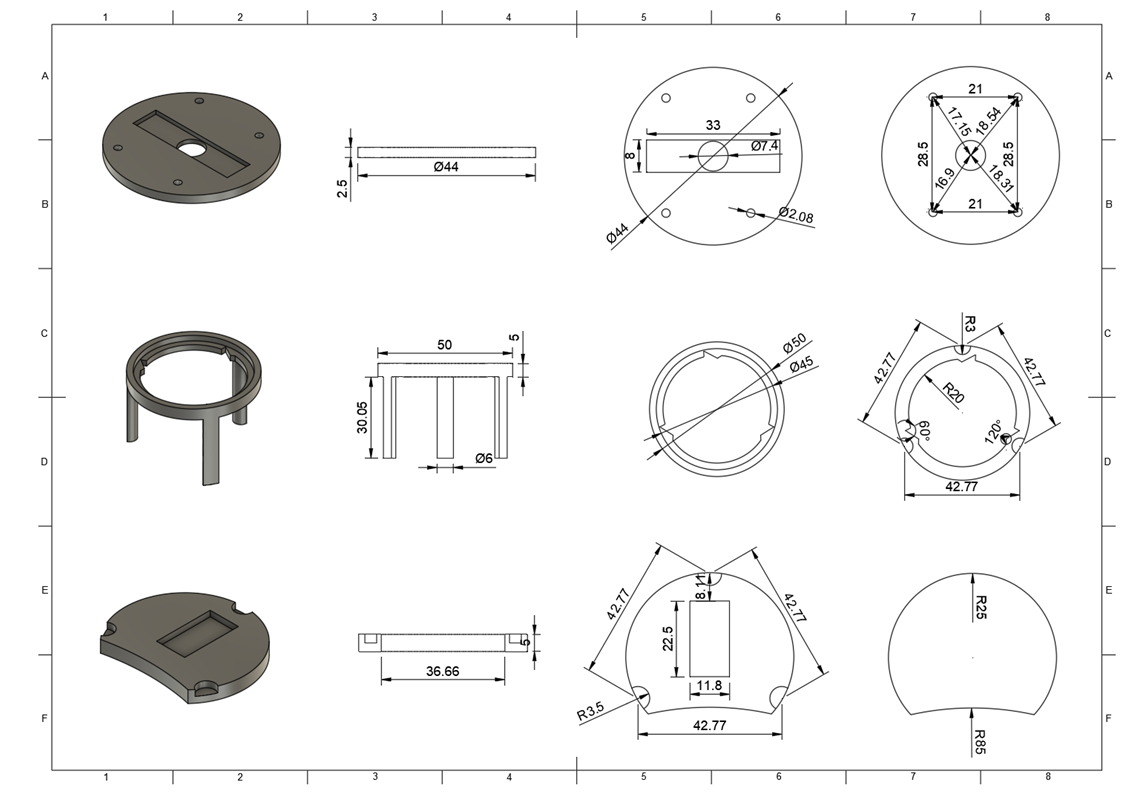
\includegraphics[width=0.9\textwidth]{figures/Armv1 (2).PNG}
    \caption{機械臂版本一設計圖紙 第二頁(單位:mm)}
\end{figure}

\begin{figure}[htbp]
    \centering
    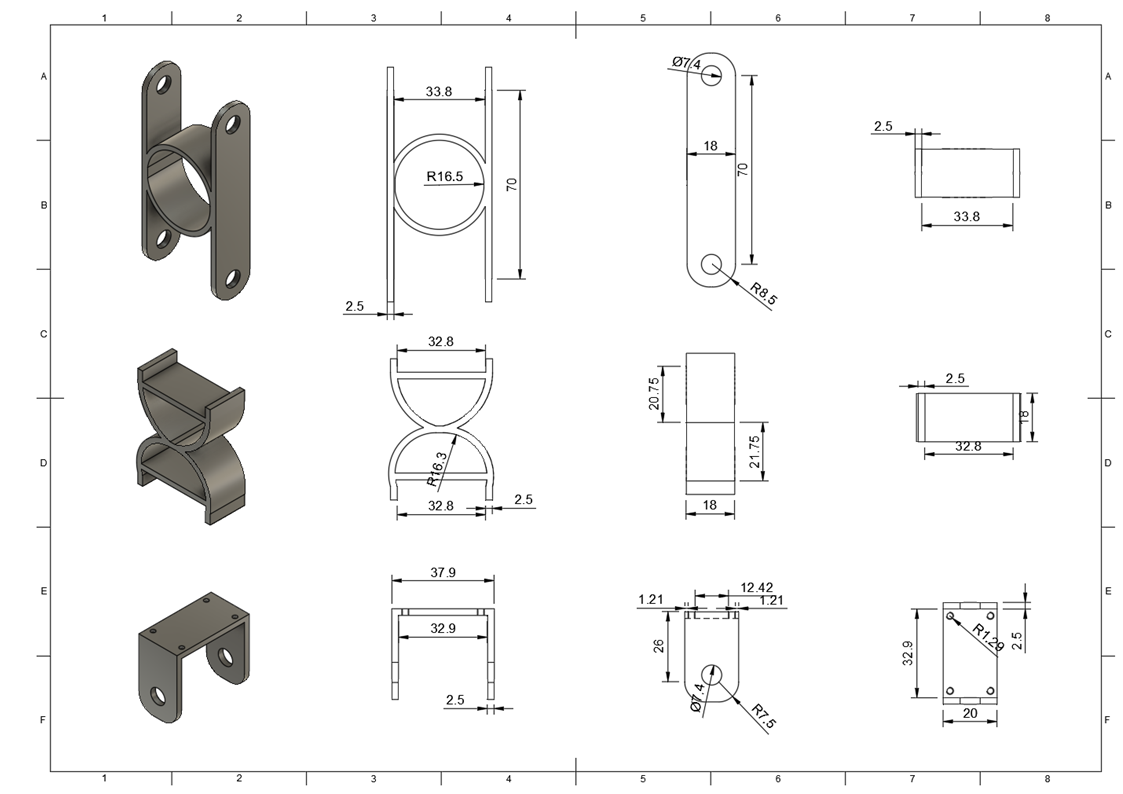
\includegraphics[width=0.9\textwidth]{figures/Armv1 (3).PNG}
    \caption{機械臂版本一設計圖紙 第三頁(單位:mm)}
\end{figure}

\begin{figure}[htbp]
    \centering
    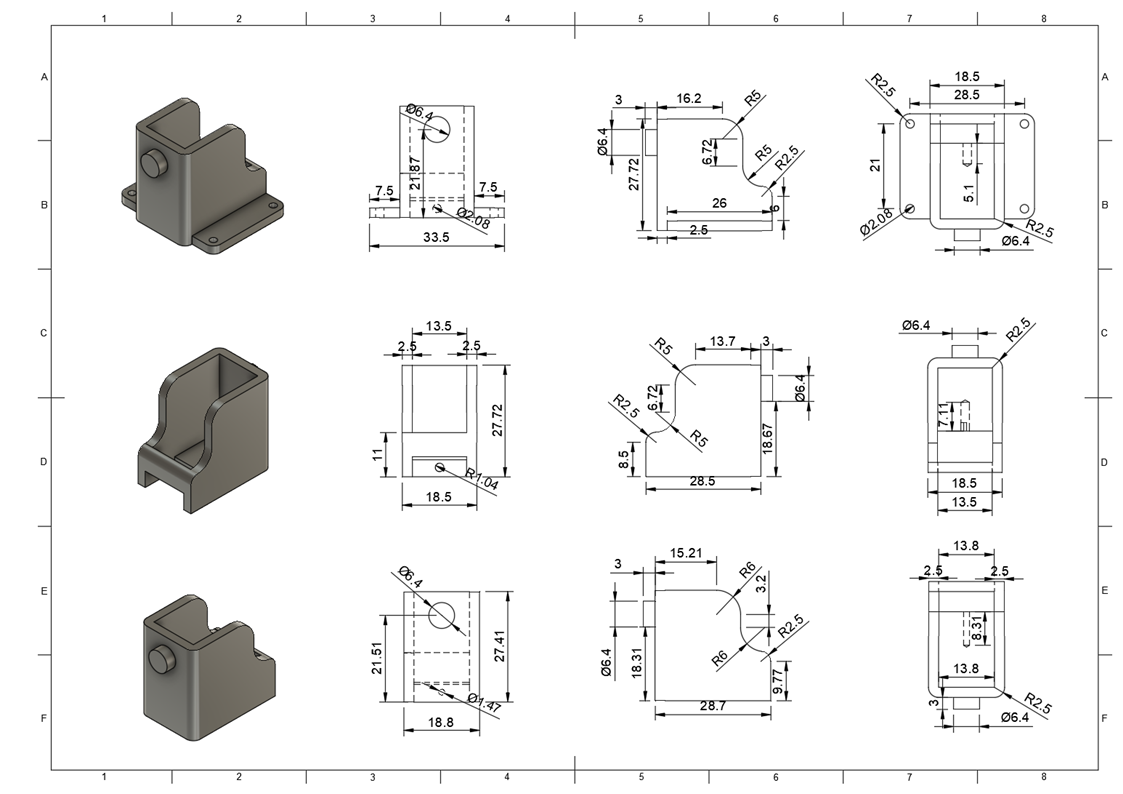
\includegraphics[width=0.9\textwidth]{figures/Armv1 (4).PNG}
    \caption{機械臂版本一設計圖紙 第四頁(單位:mm)}
\end{figure}

\begin{figure}[htbp]
    \centering
    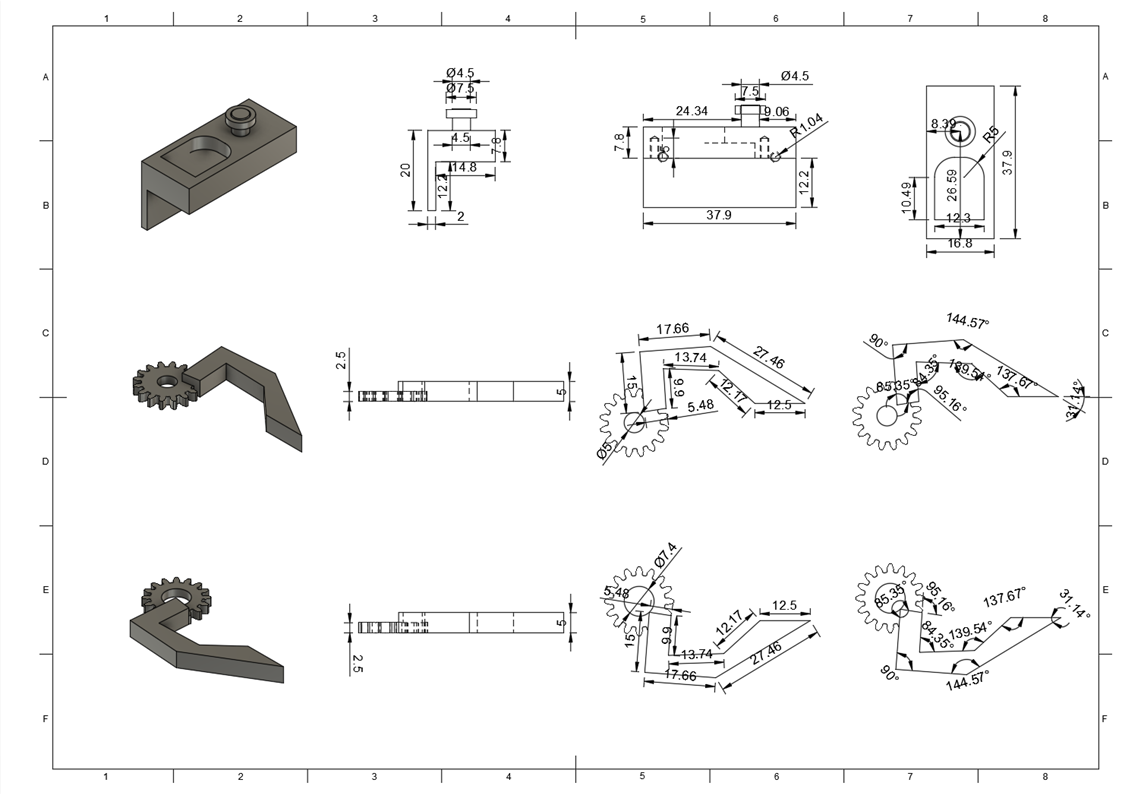
\includegraphics[width=0.9\textwidth]{figures/Armv1 (5).PNG}
    \caption{機械臂版本一設計圖紙 第五頁(單位:mm)}
\end{figure}



\section{實驗二:將機械臂用於畫圖}
\subsection{機械結構設計圖}
本實驗的硬體部分使用了3D列印技術,結合小型伺服馬達,設計了一個畫筆的小型機械臂,以下為此硬體的詳細設計圖紙:
\begin{figure}[htbp]
    \centering
    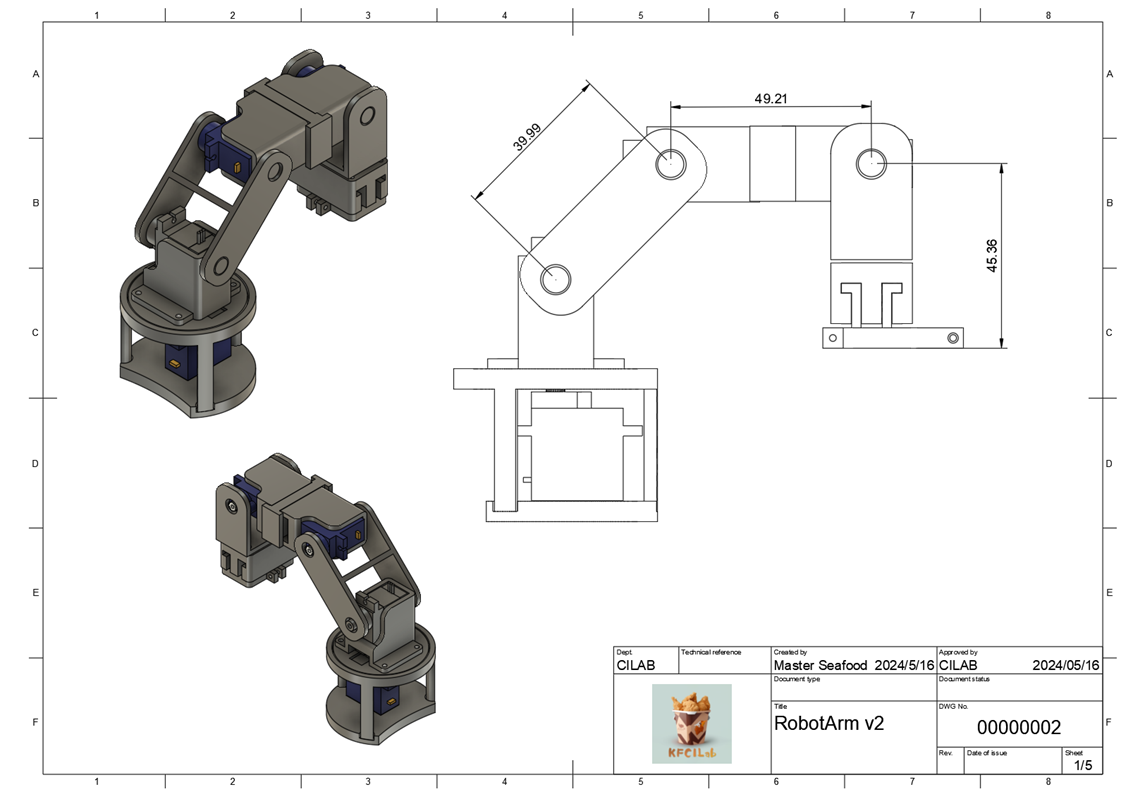
\includegraphics[width=0.9\textwidth]{figures/Armv2 (1).PNG}
    \caption{機械臂版本二設計圖紙 第一頁(單位:mm)}
    %\label{fig:Armv1Drawing_p1}}
\end{figure}

\begin{figure}[htbp]
    \centering
    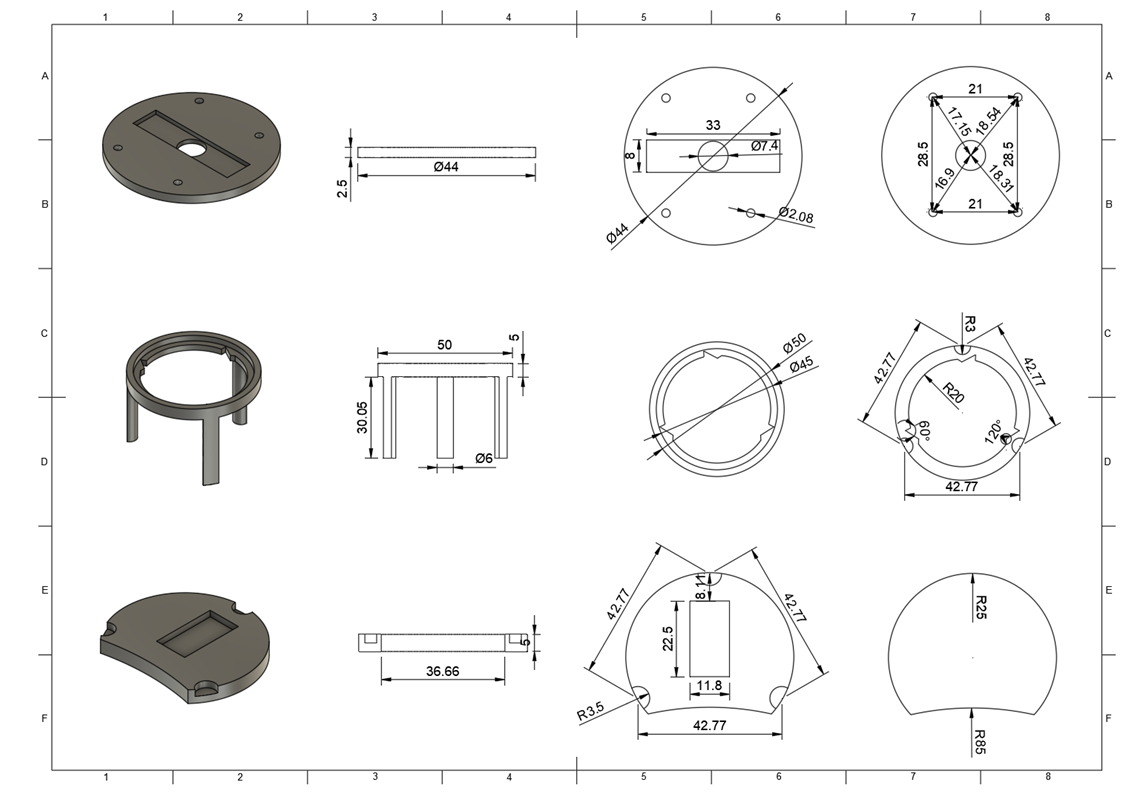
\includegraphics[width=0.9\textwidth]{figures/Armv2 (2).PNG}
    \caption{機械臂版本二設計圖紙 第二頁(單位:mm)}
\end{figure}

\begin{figure}[htbp]
    \centering
    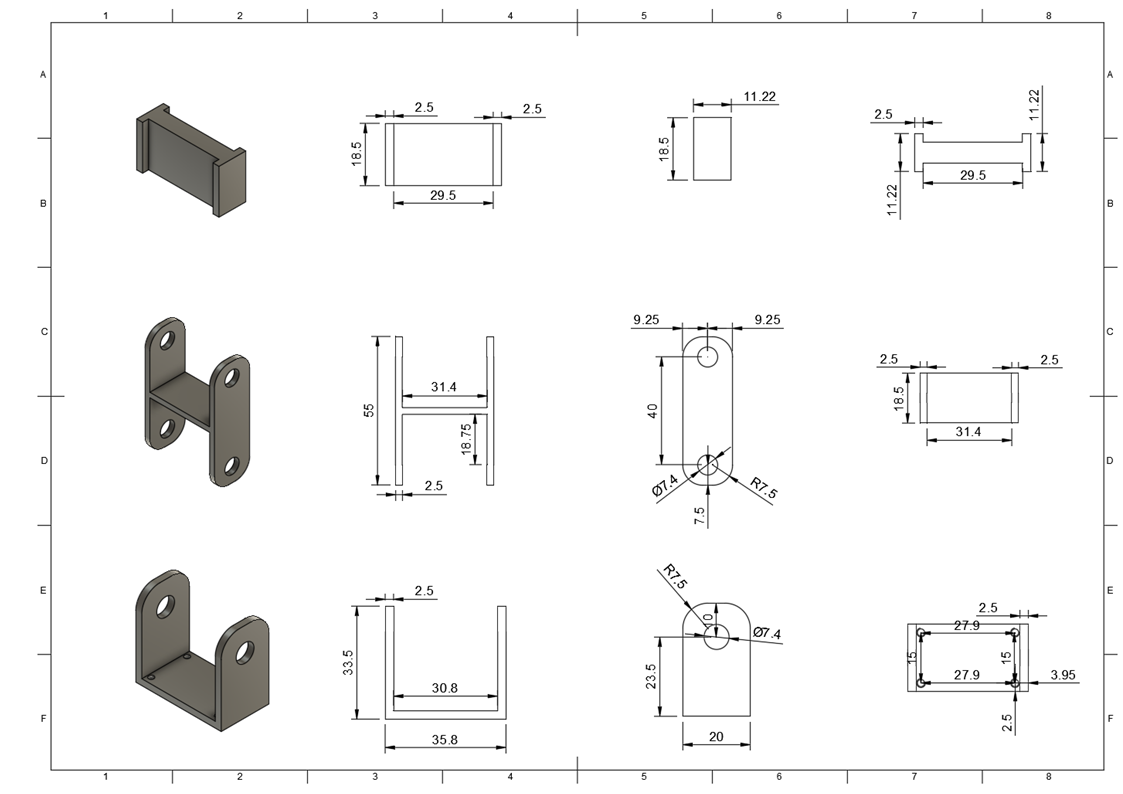
\includegraphics[width=0.9\textwidth]{figures/Armv2 (3).PNG}
    \caption{機械臂版本二設計圖紙 第三頁(單位:mm)}
\end{figure}

\begin{figure}[htbp]
    \centering
    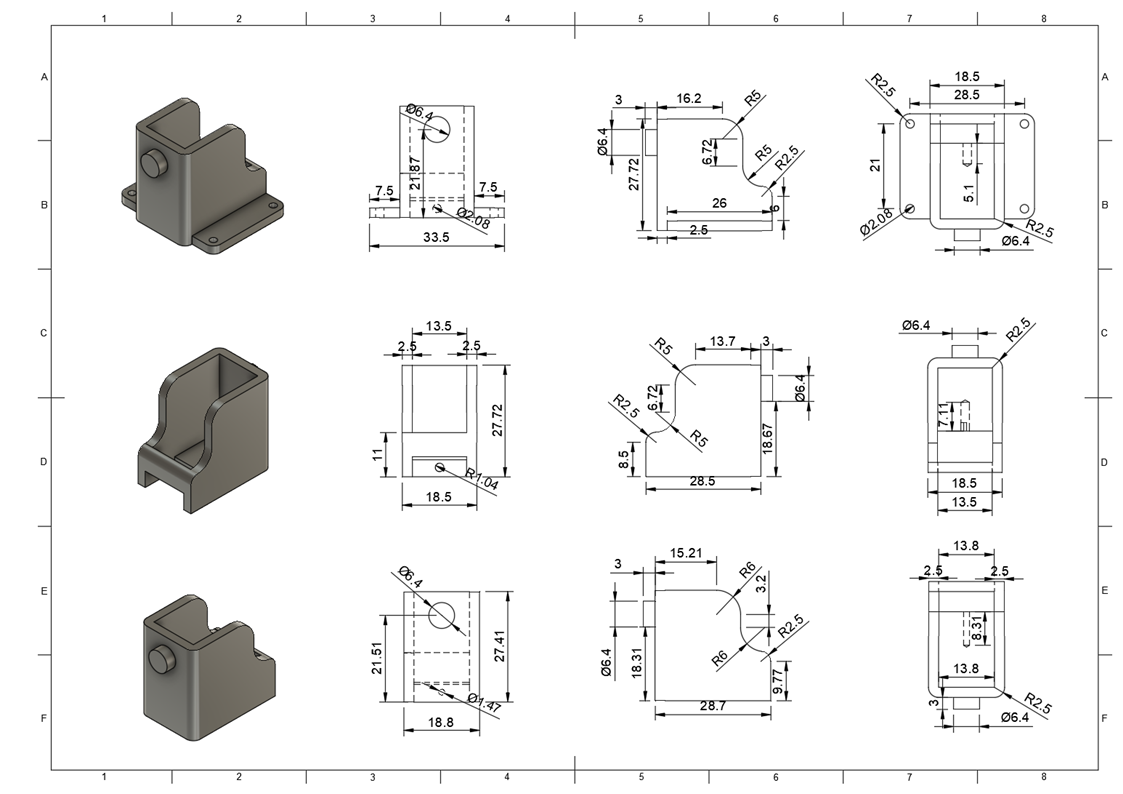
\includegraphics[width=0.9\textwidth]{figures/Armv2 (4).PNG}
    \caption{機械臂版本二設計圖紙 第四頁(單位:mm)}
\end{figure}

\begin{figure}[htbp]
    \centering
    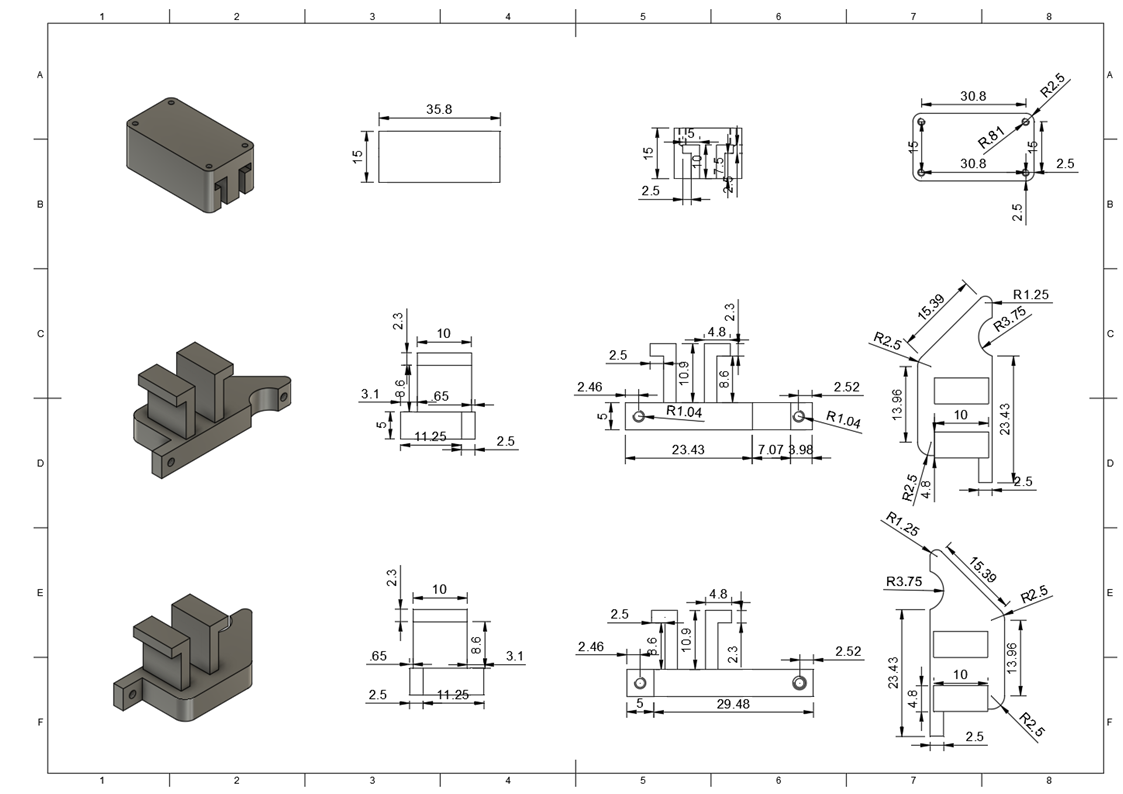
\includegraphics[width=0.9\textwidth]{figures/Armv2 (5).PNG}
    \caption{機械臂版本二設計圖紙 第五頁(單位:mm)}
\end{figure}

\section{實驗三:機械臂在自動運輸車上的應用}
\subsection{機械結構設計圖}
本實驗將機械臂與自動運輸車、鏡頭等硬體結合,設計了一台裝載機械臂的無人搬運車,以下為此硬體的詳細設計圖紙:
\begin{figure}[htbp]
    \centering
    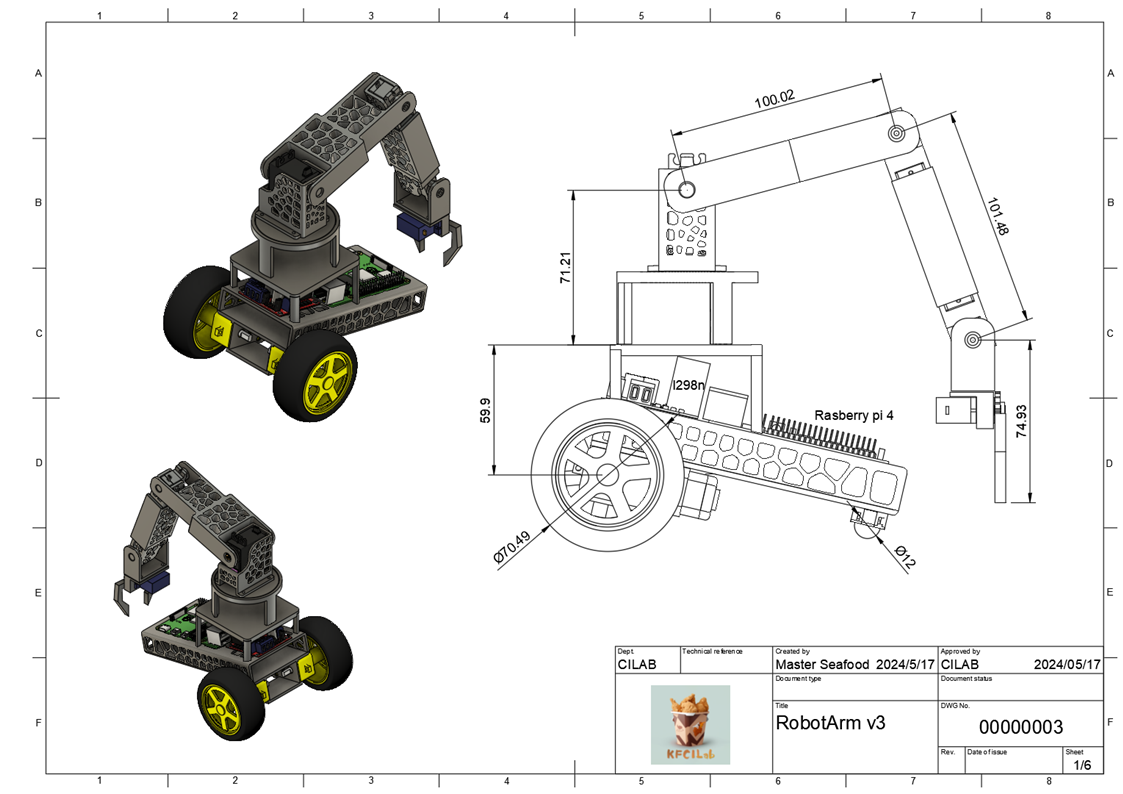
\includegraphics[width=0.9\textwidth]{figures/Armv3 (1).PNG}
    \caption{機械臂版本三設計圖紙 第一頁(單位:mm)}
    %\label{fig:Armv1Drawing_p1}}
\end{figure}

\begin{figure}[htbp]
    \centering
    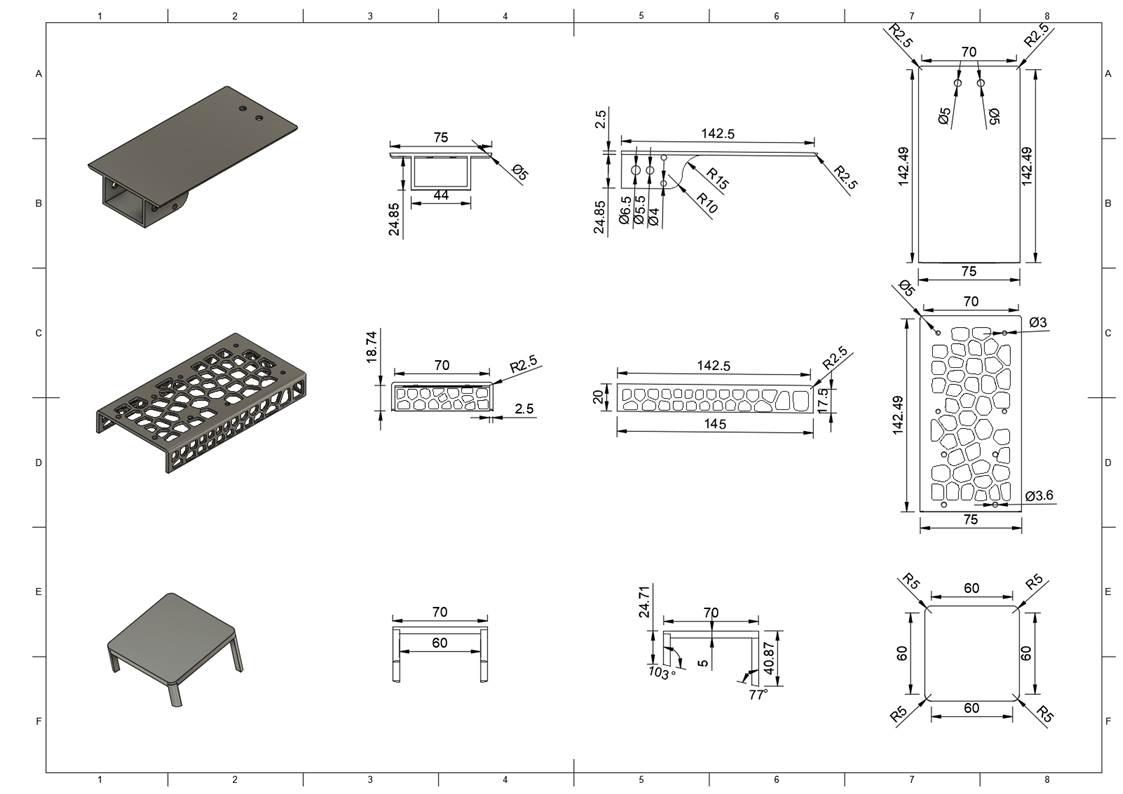
\includegraphics[width=0.9\textwidth]{figures/Armv3 (2).PNG}
    \caption{機械臂版本三設計圖紙 第二頁(單位:mm)}
\end{figure}

\begin{figure}[htbp]
    \centering
    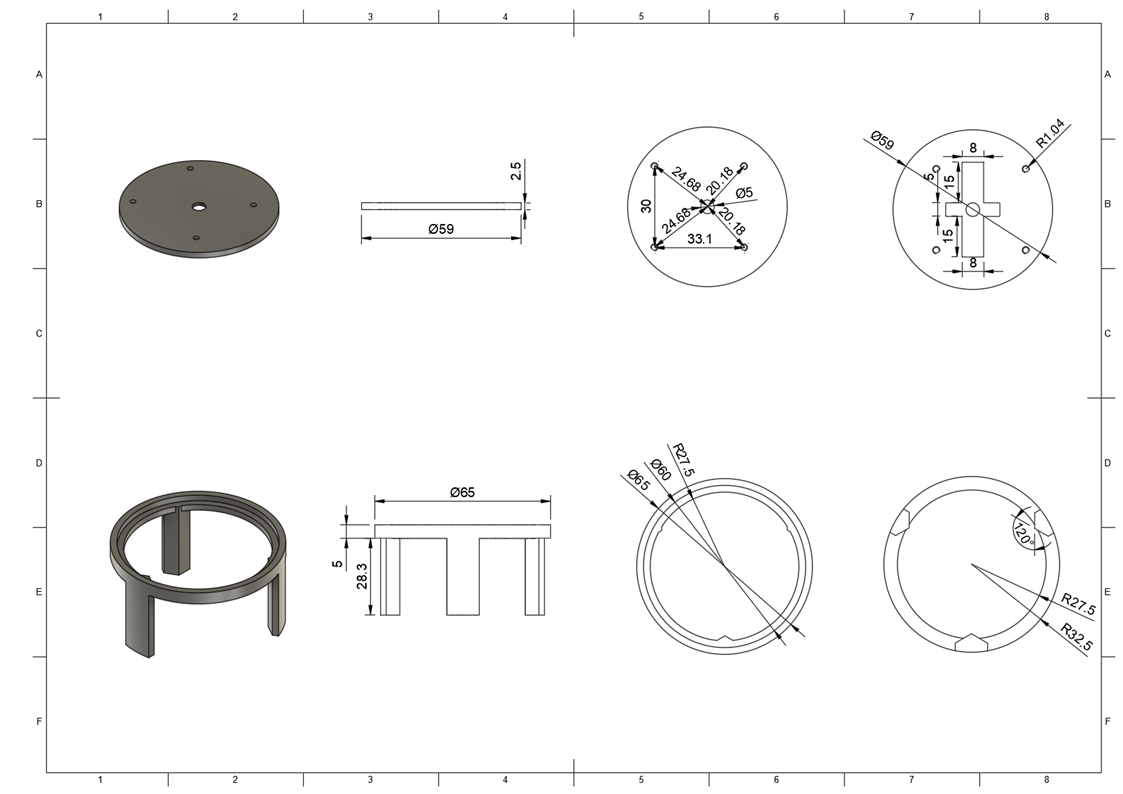
\includegraphics[width=0.9\textwidth]{figures/Armv3 (3).PNG}
    \caption{機械臂版本三設計圖紙 第三頁(單位:mm)}
\end{figure}

\begin{figure}[htbp]
    \centering
    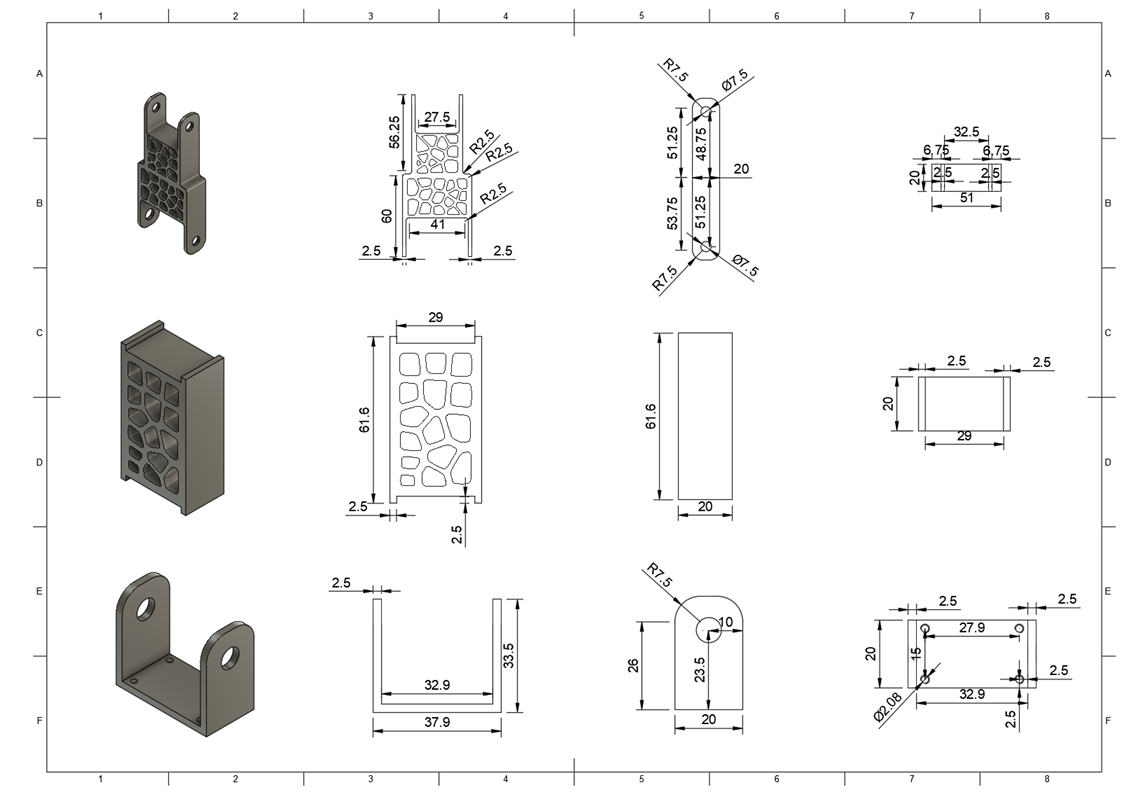
\includegraphics[width=0.9\textwidth]{figures/Armv3 (4).PNG}
    \caption{機械臂版本三設計圖紙 第四頁(單位:mm)}
\end{figure}

\begin{figure}[htbp]
    \centering
    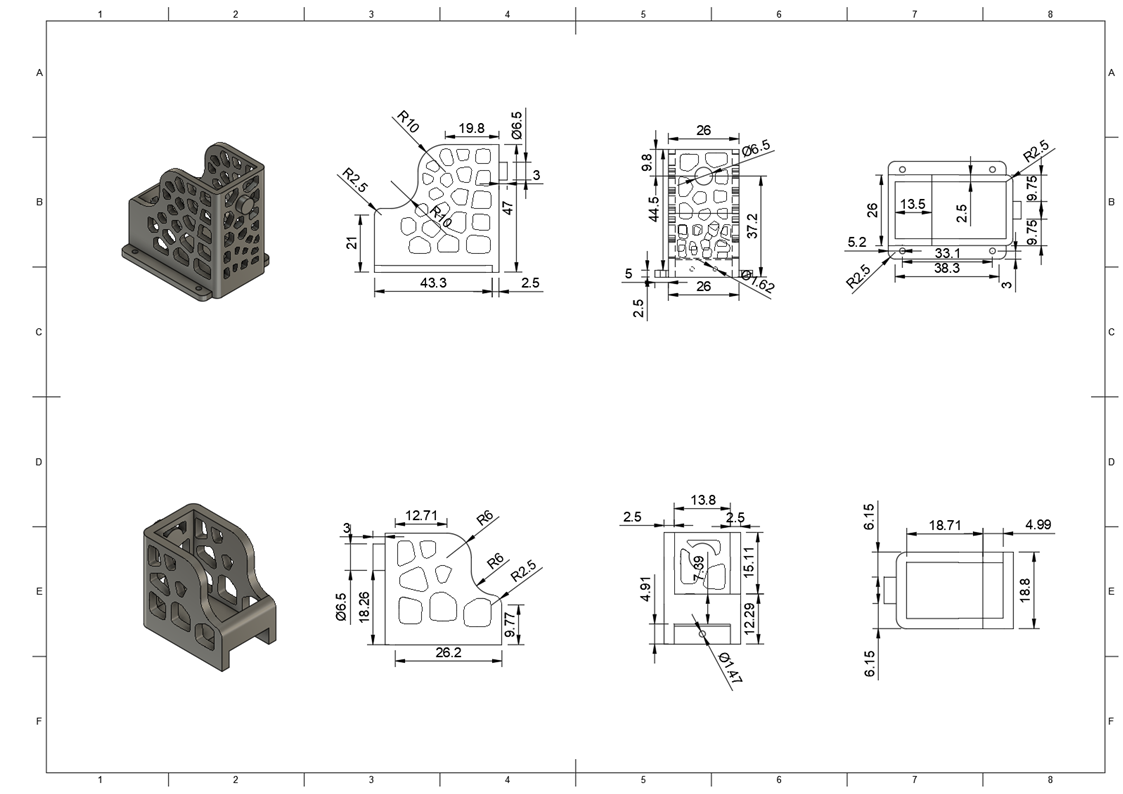
\includegraphics[width=0.9\textwidth]{figures/Armv3 (5).PNG}
    \caption{機械臂版本三設計圖紙 第五頁(單位:mm)}
\end{figure}

\begin{figure}[htbp]
    \centering
    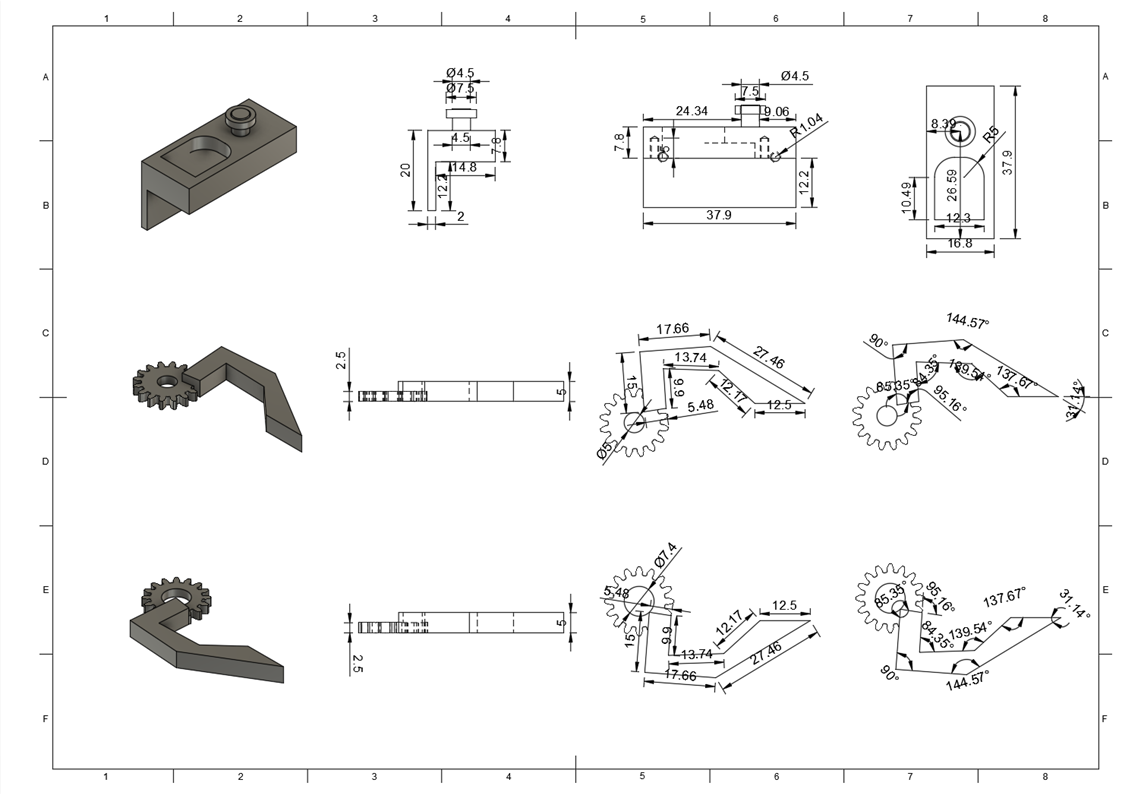
\includegraphics[width=0.9\textwidth]{figures/Armv3 (6).PNG}
    \caption{機械臂版本三設計圖紙 第六頁(單位:mm)}
\end{figure}

\subsection{函數設計}

\subsection{大型語言模型的範例輸入與輸出}
\begin{listing}
\begin{minted}[frame=single,
               framesep=3mm,
               linenos=true,
               xleftmargin=21pt,
               tabsize=4]{js}
{     
    "role": "user",
    "content" : 
    "The following functions are available:\
    aim(color): Let the robot aim at a block of a specific color.\
    color option: red, blue\
    grab: Make the robot arm grab the block and put it down.\
    reset: Return the robotic arm to its initial position\
    (needs to be executed before each aiming).\
    Please help me use the above functions to control the robot arm,\
    and do not output other text other than the above functions.\
    (Use "," to separate each step)"
},
{
    "role": "user", 
    "content": "Task: Please grab the red block, and then grab the blue block."
}
\end{minted}
\caption{指令格式範例} 
\end{listing}


\end{document}